\begin{figure}[h]
\uwsinglespace
\begin{center}
\begin{minipage}{0.8\textwidth}
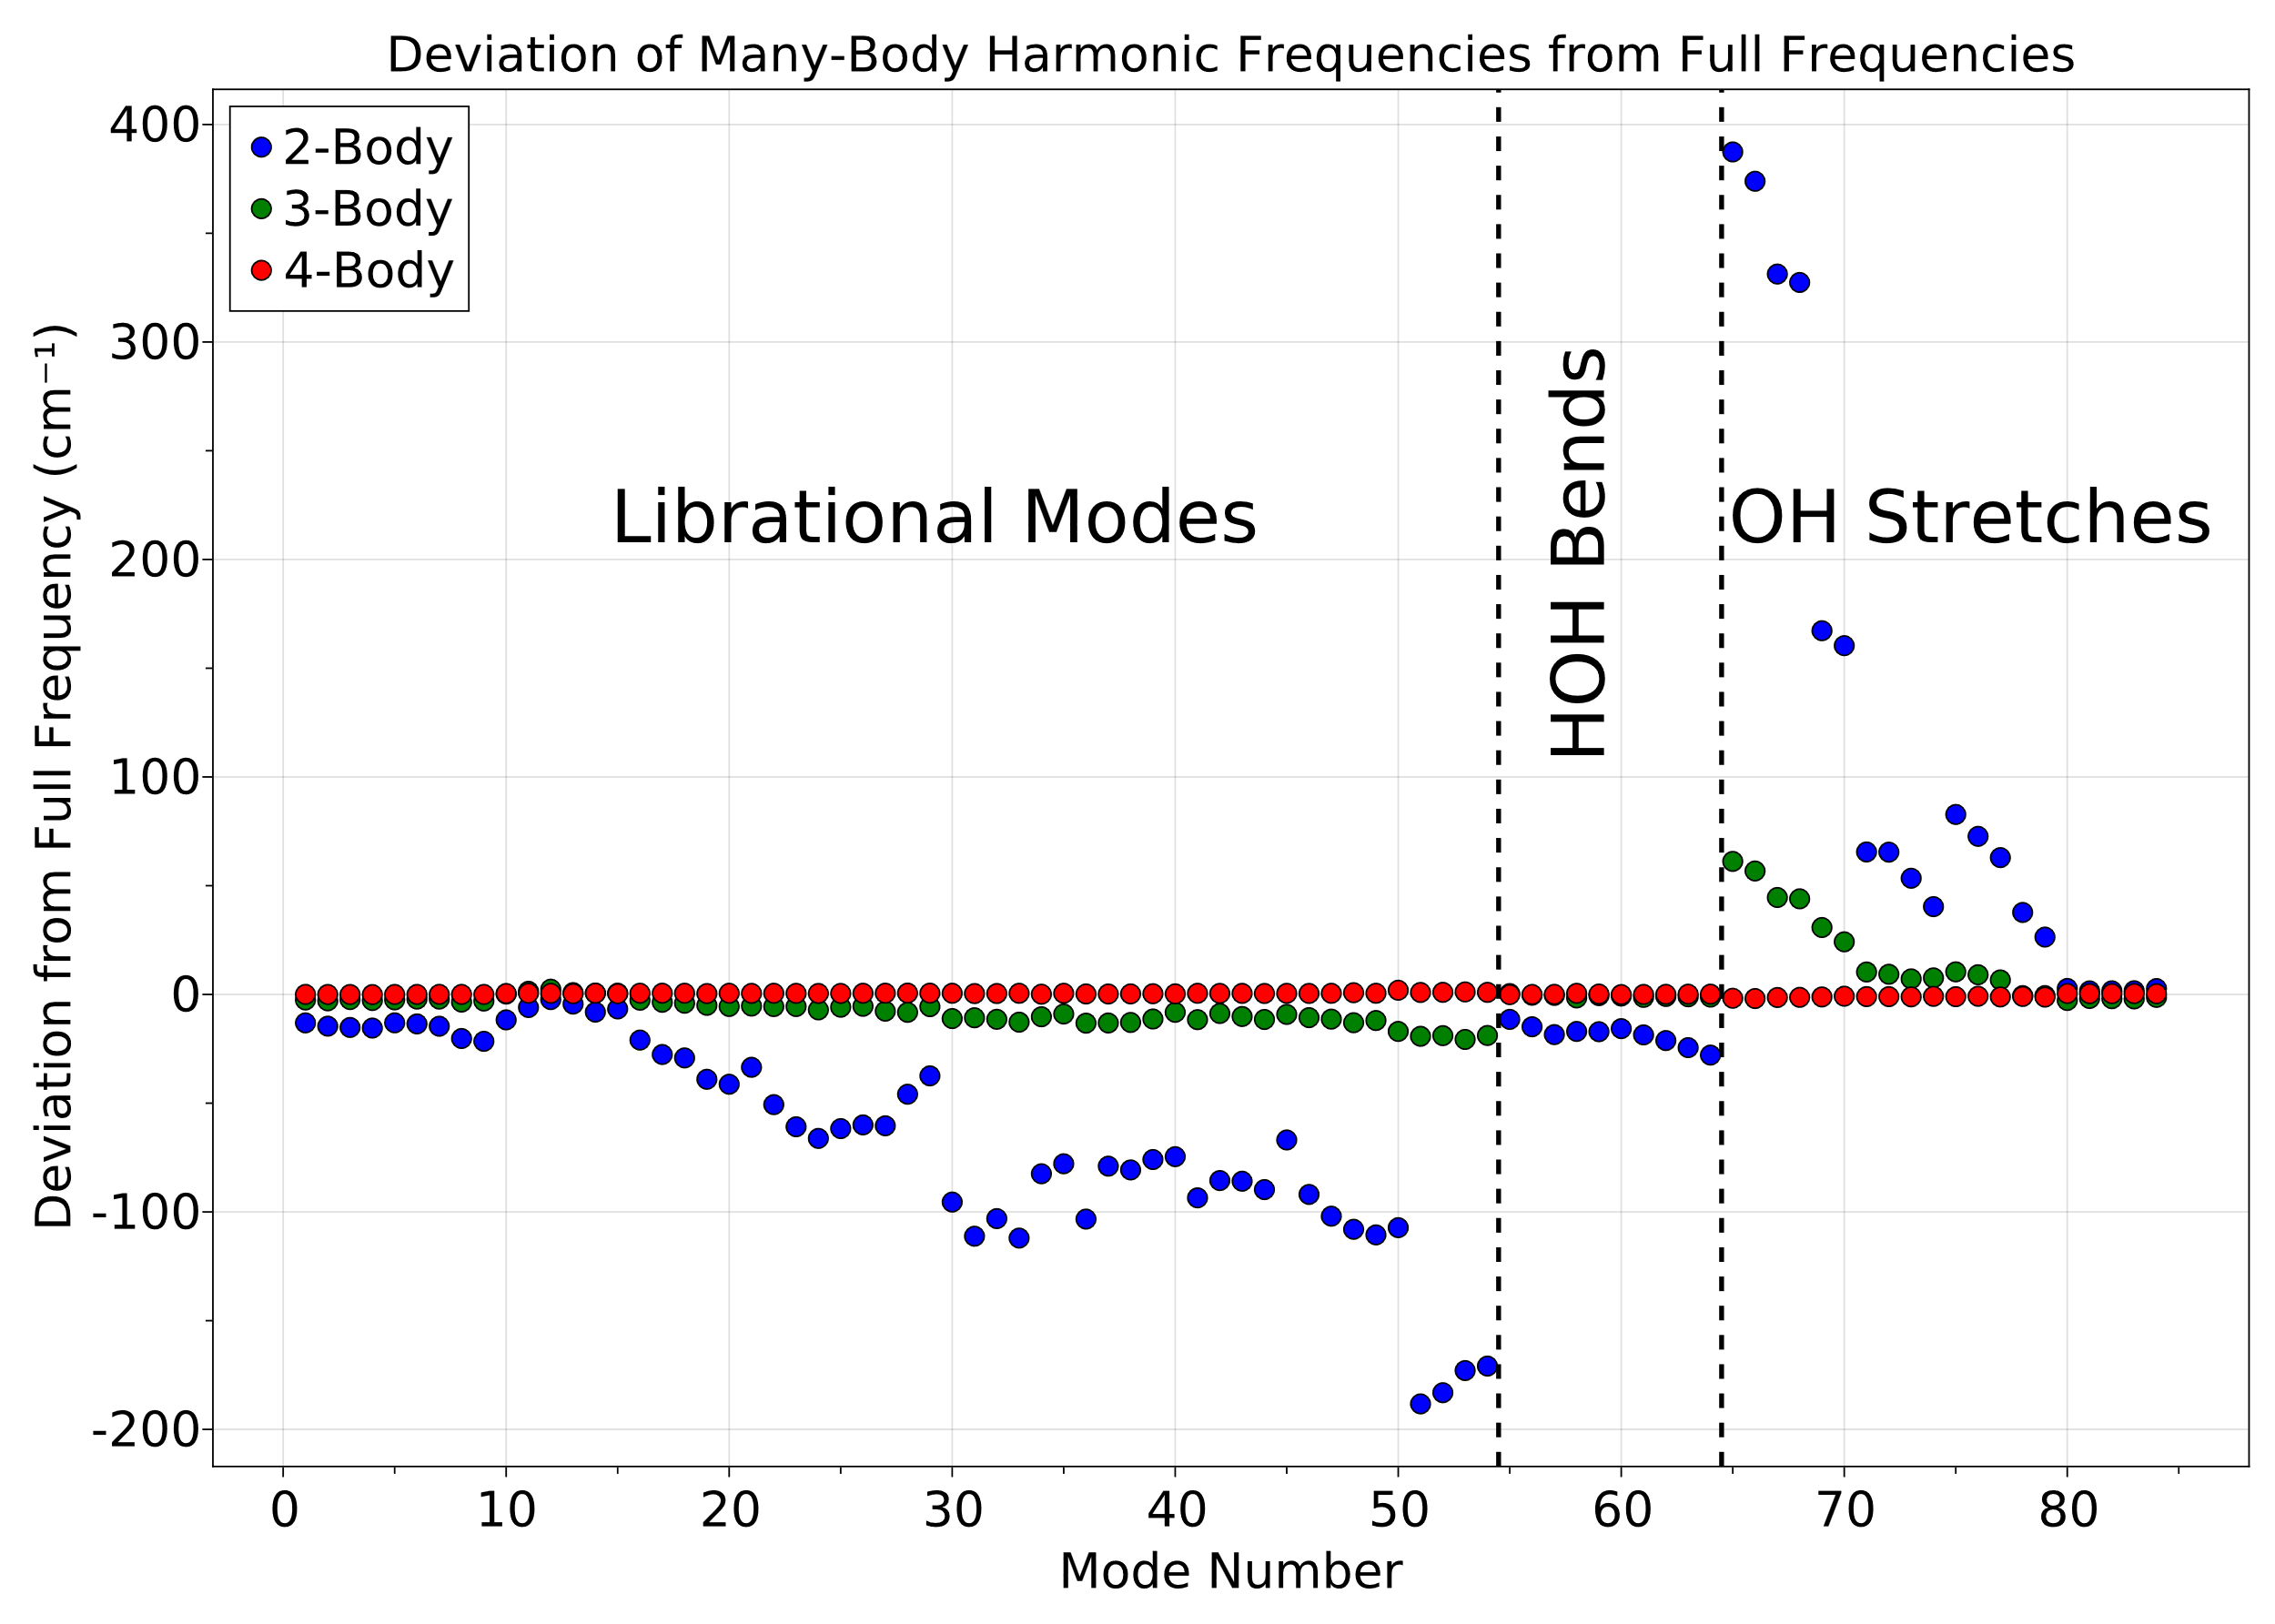
\includegraphics[width=\textwidth]{Figures/Chapter_4/ch4_figure_7.png}
\end{minipage}
\end{center}
\caption[Deviation of harmonic frequencies at 2-, 3-, and 4-body levels using the MB-Pol potential. The \ce{(H2O)_{10}} cluster of interest was re-optimized using the MBE and harmonic frequencies were calculated at each minimum using the $k$-body potential.]{Deviation of harmonic frequencies at 2-, 3-, and 4-body levels using the MB-Pol potential. The \ce{(H2O)_{10}} cluster of interest was re-optimized using the MBE and harmonic frequencies were calculated at each minimum using the $k$-body potential. The x-axis simply labels the mode number starting from the lowest frequency harmonic vibration and the y-axis shows deviation from the full harmonic frequencies. The dashed lines separate low-frequency librational modes from HOH bends and OH stretches. The 4-body representation has a maximum deviation of less than 5 $\mathrm{cm}^{-1}$ in the OH stretches.}
\label{fig:MBE_MD_F7}
\end{figure}